%Beamer class
\documentclass{beamer}

\usepackage[czech]{babel}
\usepackage[utf8]{inputenc}
\usepackage{fontenc}
\usepackage{tgheros}
\usepackage{array}
\usepackage{color}
\usepackage{hyperref}

\usetheme{Antibes}
\usecolortheme{crane}


\title[Realizace prototypu]{Realizace prototypu}
\subtitle[KEO] {Konstrukce a realizace elektronických obvodů}
\author[Brejcha]{\texorpdfstring{Michal Brejcha\newline\url{brejcmic@fel.cvut.cz}}{Michal Brejcha}}
\institute[CVUT]{ČVUT v Praze, FEL}
\date[Praha, 2018]{Praha, 2018}

%------------------------------------------------------------------------------
%Konstanty a definice
%------------------------------------------------------------------------------
\newtheorem{myDef}{}
\newcommand{\kicadVersion}{5.0.0.}

\begin{document}
%------------------------------------------------------------------------------
%Uvodni slajd
%------------------------------------------------------------------------------
\frame{\titlepage}

\begin{frame}
\frametitle{Obsah} 
\tableofcontents
\end{frame}

\AtBeginSection[]
{
  \begin{frame}
    \frametitle{Téma}
    \tableofcontents[currentsection]
  \end{frame}
}

%------------------------------------------------------------------------------
%Návrh
%------------------------------------------------------------------------------
\section{\texorpdfstring{Návrh}{Navrh}}
\subsection{\texorpdfstring{Nepájivé pole}{Nepajive pole}}
%------------------------------------------------------------------------------
  \begin{frame}
    \frametitle{Nepájivé pole - breadboard}
    \begin{center}
      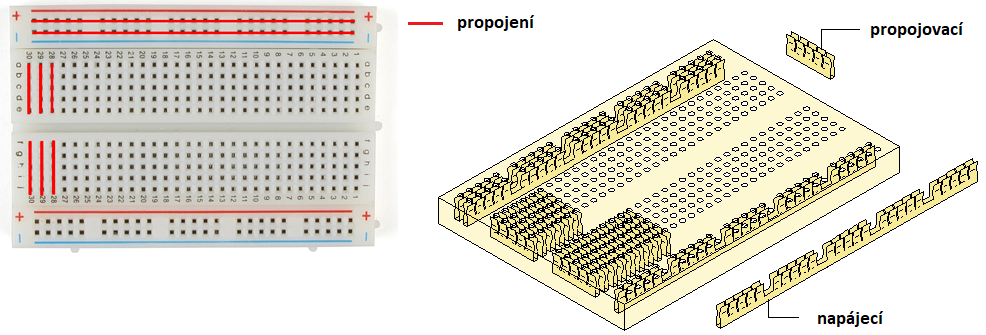
\includegraphics[width=\textwidth]{obr/breadBoard_bot.png}
    \end{center}
  \end{frame}
%------------------------------------------------------------------------------
  \begin{frame}
    \frametitle{Nepájivé pole - realizace prototypu}
    \begin{center}
      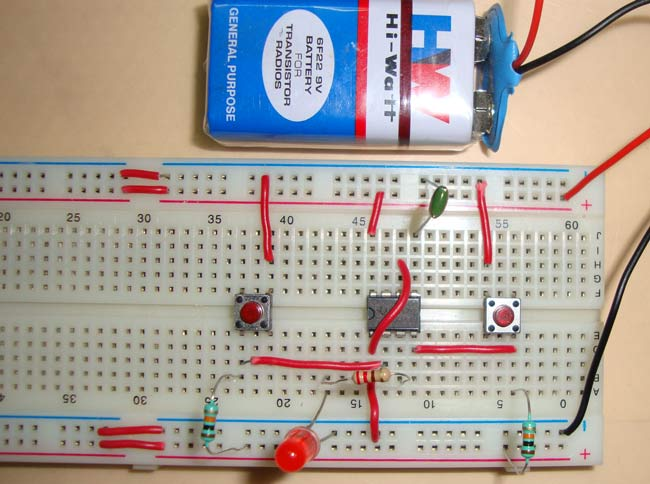
\includegraphics[width=0.8\textwidth]{obr/breadBoard_prot.png}
    \end{center}
  \end{frame}
%------------------------------------------------------------------------------
\subsection{\texorpdfstring{Prototypová deska s prokovy}{Prototypová deska s prokovy}}
%------------------------------------------------------------------------------
  \begin{frame}
    \frametitle{Prototypová deska s prokovy (pady) - perfboard}
    \begin{center}
      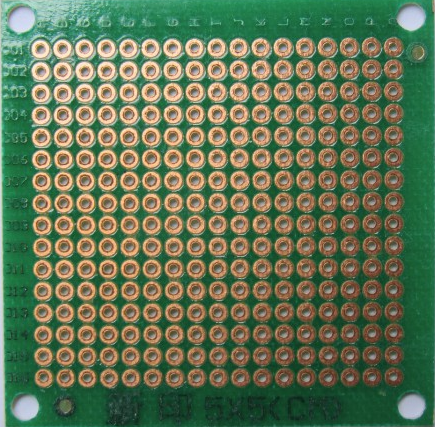
\includegraphics[width=0.5\textwidth]{obr/perfBoard_bot.png}
    \end{center}
  \end{frame}
%------------------------------------------------------------------------------
  \begin{frame}
    \frametitle{Prototypová deska s prokovy (pady) - realizace prototypu}
    \begin{center}
      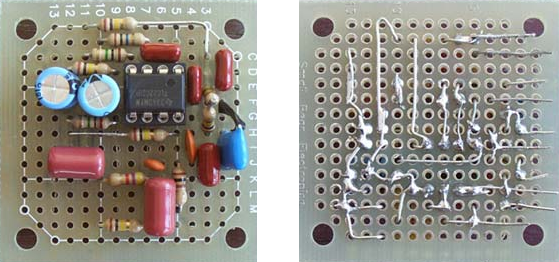
\includegraphics[width=\textwidth]{obr/perfBoard_prot.png}
    \end{center}
  \end{frame}
%------------------------------------------------------------------------------
\subsection{\texorpdfstring{Prototypová deska s pásky}{Prototypova deska s pasky}}
%------------------------------------------------------------------------------
  \begin{frame}
    \frametitle{Prototypová deska s pásky - stripboard}
    \begin{center}
      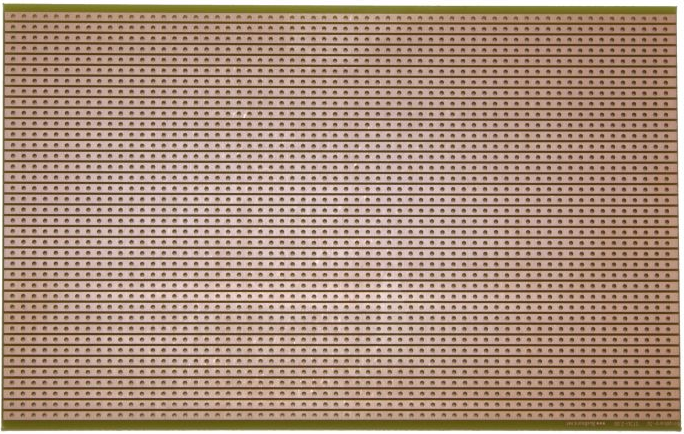
\includegraphics[width=0.8\textwidth]{obr/stripBoard_bot.png}
    \end{center}
  \end{frame}
%------------------------------------------------------------------------------
  \begin{frame}
    \frametitle{Prototypová deska s pásky - realizace prototypu}
    \begin{center}
      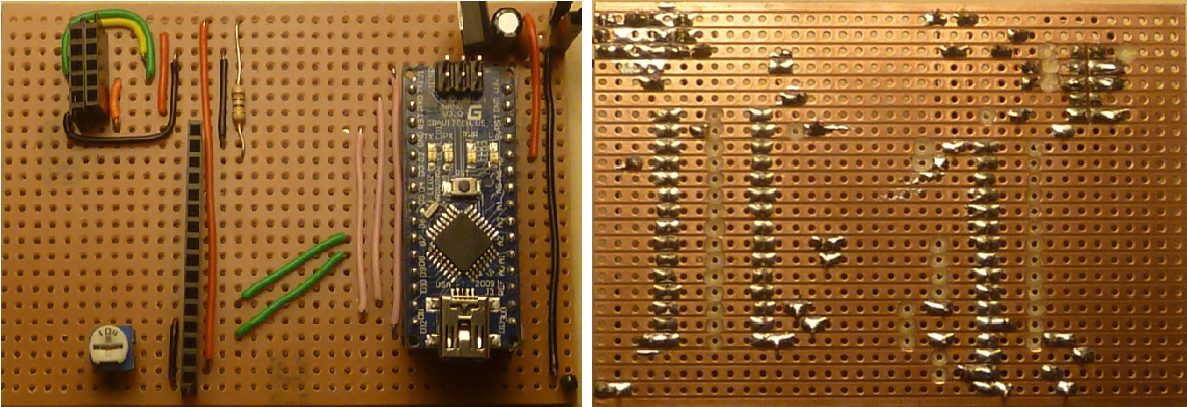
\includegraphics[width=\textwidth]{obr/stripBoard_prot.png}
    \end{center}
  \end{frame}
%------------------------------------------------------------------------------
  \begin{frame}
    \frametitle{Prototypová deska s pásky - návrh}
    \begin{center}
      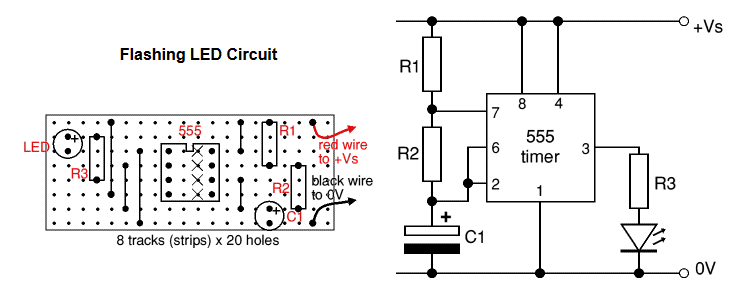
\includegraphics[width=\textwidth]{obr/stripBoard_desgn.png}
    \end{center}
  \end{frame}
%------------------------------------------------------------------------------
%------------------------------------------------------------------------------
%Součástky
%------------------------------------------------------------------------------
\section{\texorpdfstring{Součástky}{Soucastky}}
%------------------------------------------------------------------------------
  \begin{frame}
    \frametitle{Pasivní prvky}
    \begin{columns}
    
    \column{.5\textwidth}
    \begin{itemize}
      \item \textbf{Rezistory}:
        \begin{itemize}
          \item odpor,
          \item ztrátový výkon,
          \item tolerance.
        \end{itemize}
        
      \item \textbf{Kondenzátory}:
        \begin{itemize}
          \item kapacita,
          \item jmenovité napětí, 
          \item materiál (teplotní závislost),
          \item ztrátový činitel,
          \item frekvenční rozsah použití.
        \end{itemize}
    \end{itemize}
    
    \column{.5\textwidth}
    \begin{itemize}
      \item \textbf{Tlumivky, cívky:}
        \begin{itemize}
          \item indukčnost,
          \item činitel jakosti (parazitní odpor),
          \item jmenovitý proud, 
          \item frekvenční rozsah použití.
        \end{itemize}
    \end{itemize}
    \end{columns}
  \end{frame}
%------------------------------------------------------------------------------
  \begin{frame}
    \frametitle{Pouzdra rezistorů}
    \begin{center}
      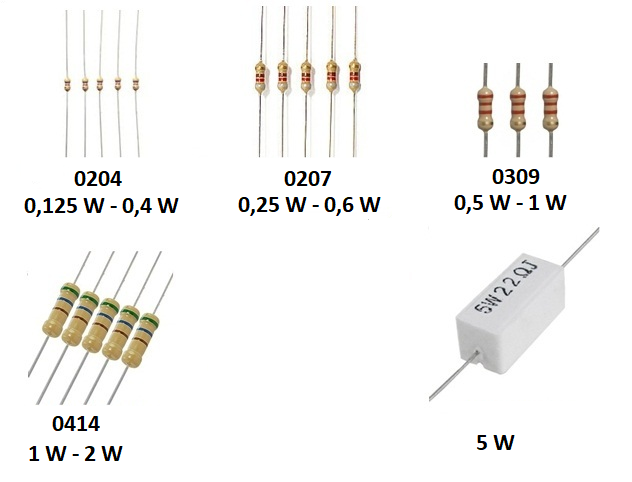
\includegraphics[width=0.8\textwidth]{obr/resistor-wattage.png}
    \end{center}
  \end{frame}
%------------------------------------------------------------------------------
  \begin{frame}
    \frametitle{Značení keramických kondenzátorů, třída 2}
    \begin{center}
      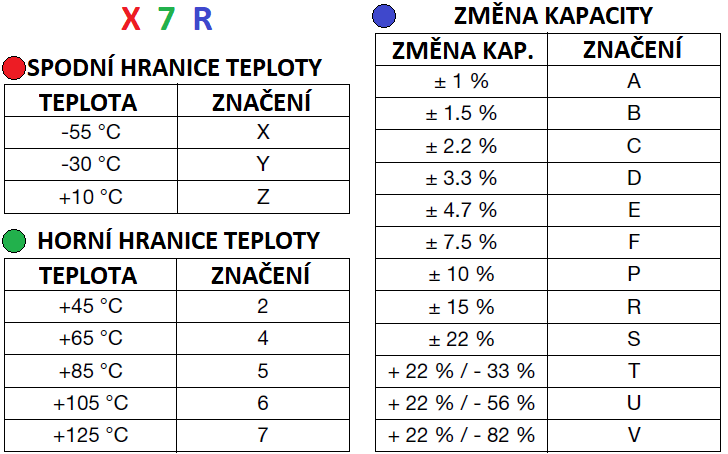
\includegraphics[width=\textwidth]{obr/classII.png}
    \end{center}
  \end{frame}
%------------------------------------------------------------------------------
  \begin{frame}
    \frametitle{Příklad - spojování prvků}
    
    \begin{itemize}
      \item Dva rezistory $R_1 = 15 \Omega$, $R_2 = 150 \Omega$  jsou spojeny 
      paralelně, na kterém je vyšší výkonová ztráta?
      \item Dva rezistory $R_1 = 15 \Omega$, $R_2 = 150 \Omega$  jsou spojeny 
      sériově, na kterém je vyšší výkonová ztráta?
      \item Dva kondenzátory $C_1 = 1 nF$, $R_2 = 10 nF$  jsou spojeny 
      sériově, na kterém je vyšší napětí?
    \end{itemize}
    
  \end{frame}
%------------------------------------------------------------------------------
  \begin{frame}
    \frametitle{Aktivní prvky}
    \begin{columns}
    
    \column{.5\textwidth}
    \begin{itemize}
      \item \textbf{Diody}:
        \begin{itemize}
          \item propustný proud,
          \item závěrné napětí,
          \item prahové napětí,
          \item doba závěrného zotavení,
          \item kapacita.
        \end{itemize}
      
      \item \textbf{Integrované obvody:}
        \begin{itemize}
          \item napájecí napětí,
          \item charakteristiky vstupů: napětí, proud, impedance,
          \item charakteristiky výstupů: napětí, proud, typ zátěže, spínací časy...
        \end{itemize}
    \end{itemize}
    
    \column{.5\textwidth}
    \begin{itemize}
      \item \textbf{Tranzistory}:
        \begin{itemize}
          \item proud kolektorem (drainem),
          \item napětí mezi kolektor-emitor (drain-source), 
          \item zesilovací činitel (převodní admitance),
          \item ztrátový výkon,
          \item frekvenční rozsah použití.
        \end{itemize}
    \end{itemize}
    \end{columns}
  \end{frame}
%------------------------------------------------------------------------------
  \begin{frame}
    \frametitle{Příklad - spojování prvků}
    
    \begin{itemize}
      \item Rezistor $R_1 = 1,1 k\Omega$ a dioda 1N4007  jsou spojeny 
      sériově a připojeny ke zdroji napětí 12 V. Jaký proud teče obvodem?
      \item Jaký rezistor se má zvolit do série k LED BL-BD0141 při napájecím
      napětí 5~V pro zvolený proud 10~mA?
      \item Jaký rezistor se má zvolit do série k LED BL-BD0141 při napájecím
      napětí 10~V se střídou 50\% pro zvolený proud 10~mA?
      \item Jaký rezistor se má zvolit do série s bází tranzistoru BC546B, tak
      aby spolehlivě sepnul (saturace) kolektorovou zátěž o velikosti 
      $R = 100\Omega$ v zapojení SE při napájecím napětí 5~V?
    \end{itemize}
    
  \end{frame}
%------------------------------------------------------------------------------
\section{\texorpdfstring{Prezetace zadání}{Prezentace zadani}}
%------------------------------------------------------------------------------
  \begin{frame}
    \frametitle{Vlastnosti prezentace}
		
		\begin{enumerate}
			\item Forma:
				\begin{itemize}
					\item Maximálně 3 slajdy nebo popis na maximálně 2 strany A4,
					\item odevzdávejte jako PDF soubor do moodle,
					\item Obsah: co chci dělat, jaké jsou parametry obvodu nebo jaké očekávám, referenční zapojení.
				\end{itemize}
			\item Důvod:
				\begin{itemize}
					\item Seznámení ostatních s projektem, který chcete realizovat $\Longrightarrow$ nutnost prezentace.
					\item Odevzdání prezentace do moodle zajistí, že vyučující bude mít přehled o tématech projektů.
				\end{itemize}
		\end{enumerate}
		\vspace{4mm}

  \end{frame}
%------------------------------------------------------------------------------
  \begin{frame}
    \frametitle{Moodle}
    \begin{center}
      
\includegraphics[width=\textwidth]{obr/moodle_ukoly.png}
    \end{center}
  \end{frame}
%------------------------------------------------------------------------------
	\begin{frame}
    \frametitle{Ukázka prezentace - Vojtěch Nydrle}
		
		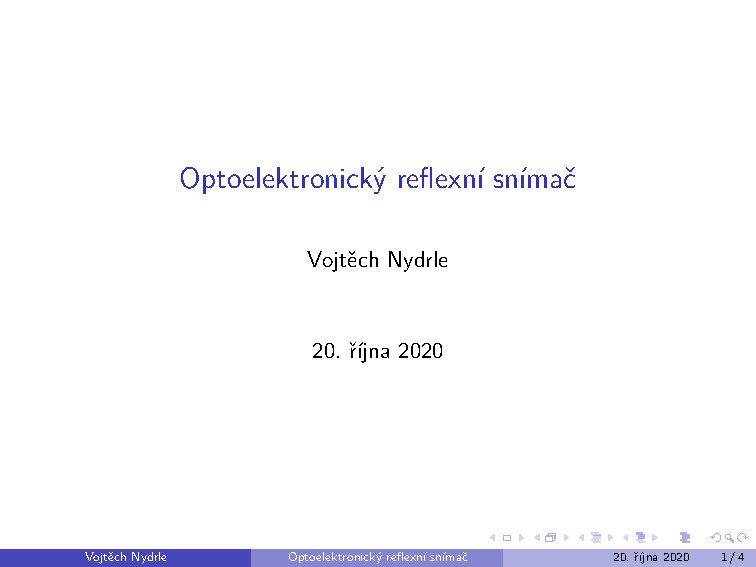
\includegraphics[page=1,width=0.9\textwidth]{pdf/prezentace_Vojtech_Nydrle.pdf}
	
	\end{frame}
%------------------------------------------------------------------------------
	\begin{frame}
    \frametitle{Ukázka prezentace - Vojtěch Nydrle}
		
		\includegraphics[page=2,width=0.9\textwidth]{pdf/prezentace_Vojtech_Nydrle.pdf}
	
	\end{frame}
%------------------------------------------------------------------------------
	\begin{frame}
    \frametitle{Ukázka prezentace - Vojtěch Nydrle}
		
		\includegraphics[page=3,width=0.9\textwidth]{pdf/prezentace_Vojtech_Nydrle.pdf}
	
	\end{frame}
%------------------------------------------------------------------------------
	\begin{frame}
    \frametitle{Ukázka prezentace - Vojtěch Nydrle}
		
		\includegraphics[page=4,width=0.9\textwidth]{pdf/prezentace_Vojtech_Nydrle.pdf}
	
	\end{frame}
%------------------------------------------------------------------------------
	\begin{frame}
    \frametitle{Ukázka stránky A4 - Šimon Hykl}
		
		
\includegraphics[scale=0.5]{obr/A4_Hykl1.png}
	
	\end{frame}
%------------------------------------------------------------------------------
	\begin{frame}
    \frametitle{Ukázka stránky A4 - Šimon Hykl}
		
		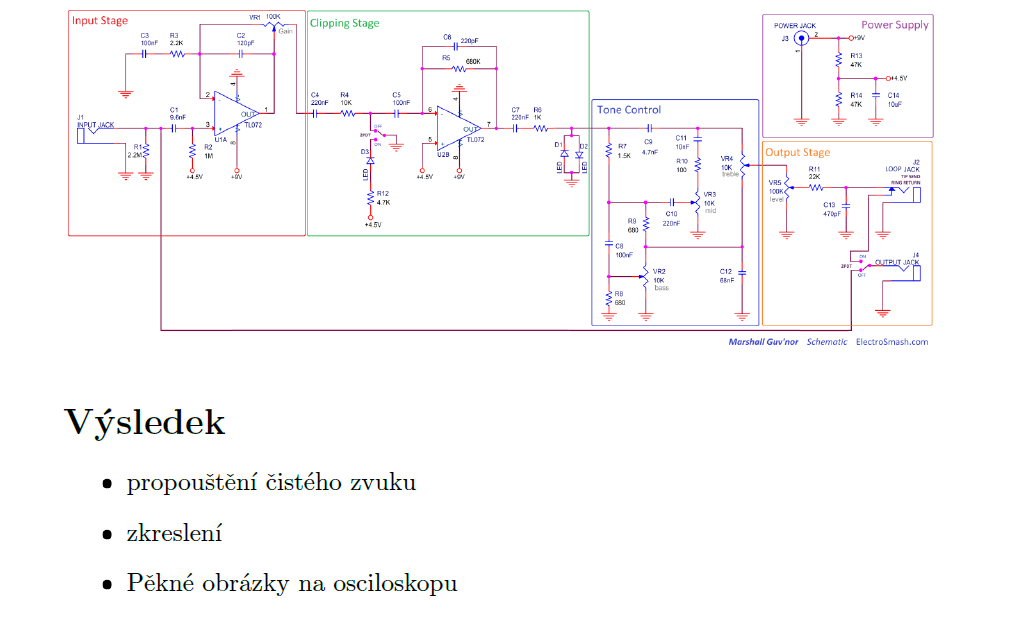
\includegraphics[scale=0.5]{obr/A4_Hykl2.png}
	
	\end{frame}
%------------------------------------------------------------------------------
  \begin{frame}
    \frametitle{Co bude příště}
    
    \begin{itemize}
      \item Prezentace vašich obvodů,
			\item rozhodneme, kterou část obvodu by bylo vhodné odzkoušet jako prototyp,
      \item příprava na KiCAD - kde ho stáhnout, instalace atd.
    \end{itemize}
    
  \end{frame}
%------------------------------------------------------------------------------
\end{document}